\newpage
\section{Управление движением робота}
\subsection{Кинематическая модель}
Кинематическая модель робота имеет вид~\cite{survey}:
\begin{equation}\label{eq_robot_kinematic_model}
    \left\{
    \begin{aligned}
        & \dot{x} = v \cos \theta \\
        & \dot{y} = v \sin \theta \\
        & \dot{\theta} = \omega
    \end{aligned}
    \right.
\end{equation}
где $x$, $y$~--- декартовы координаты точки~$C$, являющейся серединой задней оси (см.~рисунок~\ref{img_kinematic_model_picture}); $\theta$~--- угол поворота робота (угол между осями абсцисс неподвижной системы координат $Ox_0y_0$ и системы координат $Ox_1y_1$, жёстко связанной с роботом); $v$~--- проекция скорости~$\vec{v}$ точки~$C$ на ось абсцисс системы координат~$Ox_1y_1$\!\footnote{В~данной работе проскальзывание задних колес робота считается отсутствующим, а, следовательно, вектор $\vec{v}$~--- всегда коллинеарным оси абсцисс системы координат~$Ox_1y_1$.}; $\omega$~--- угловая скорость вращения робота.

\begin{figure}[h]
    \centering
    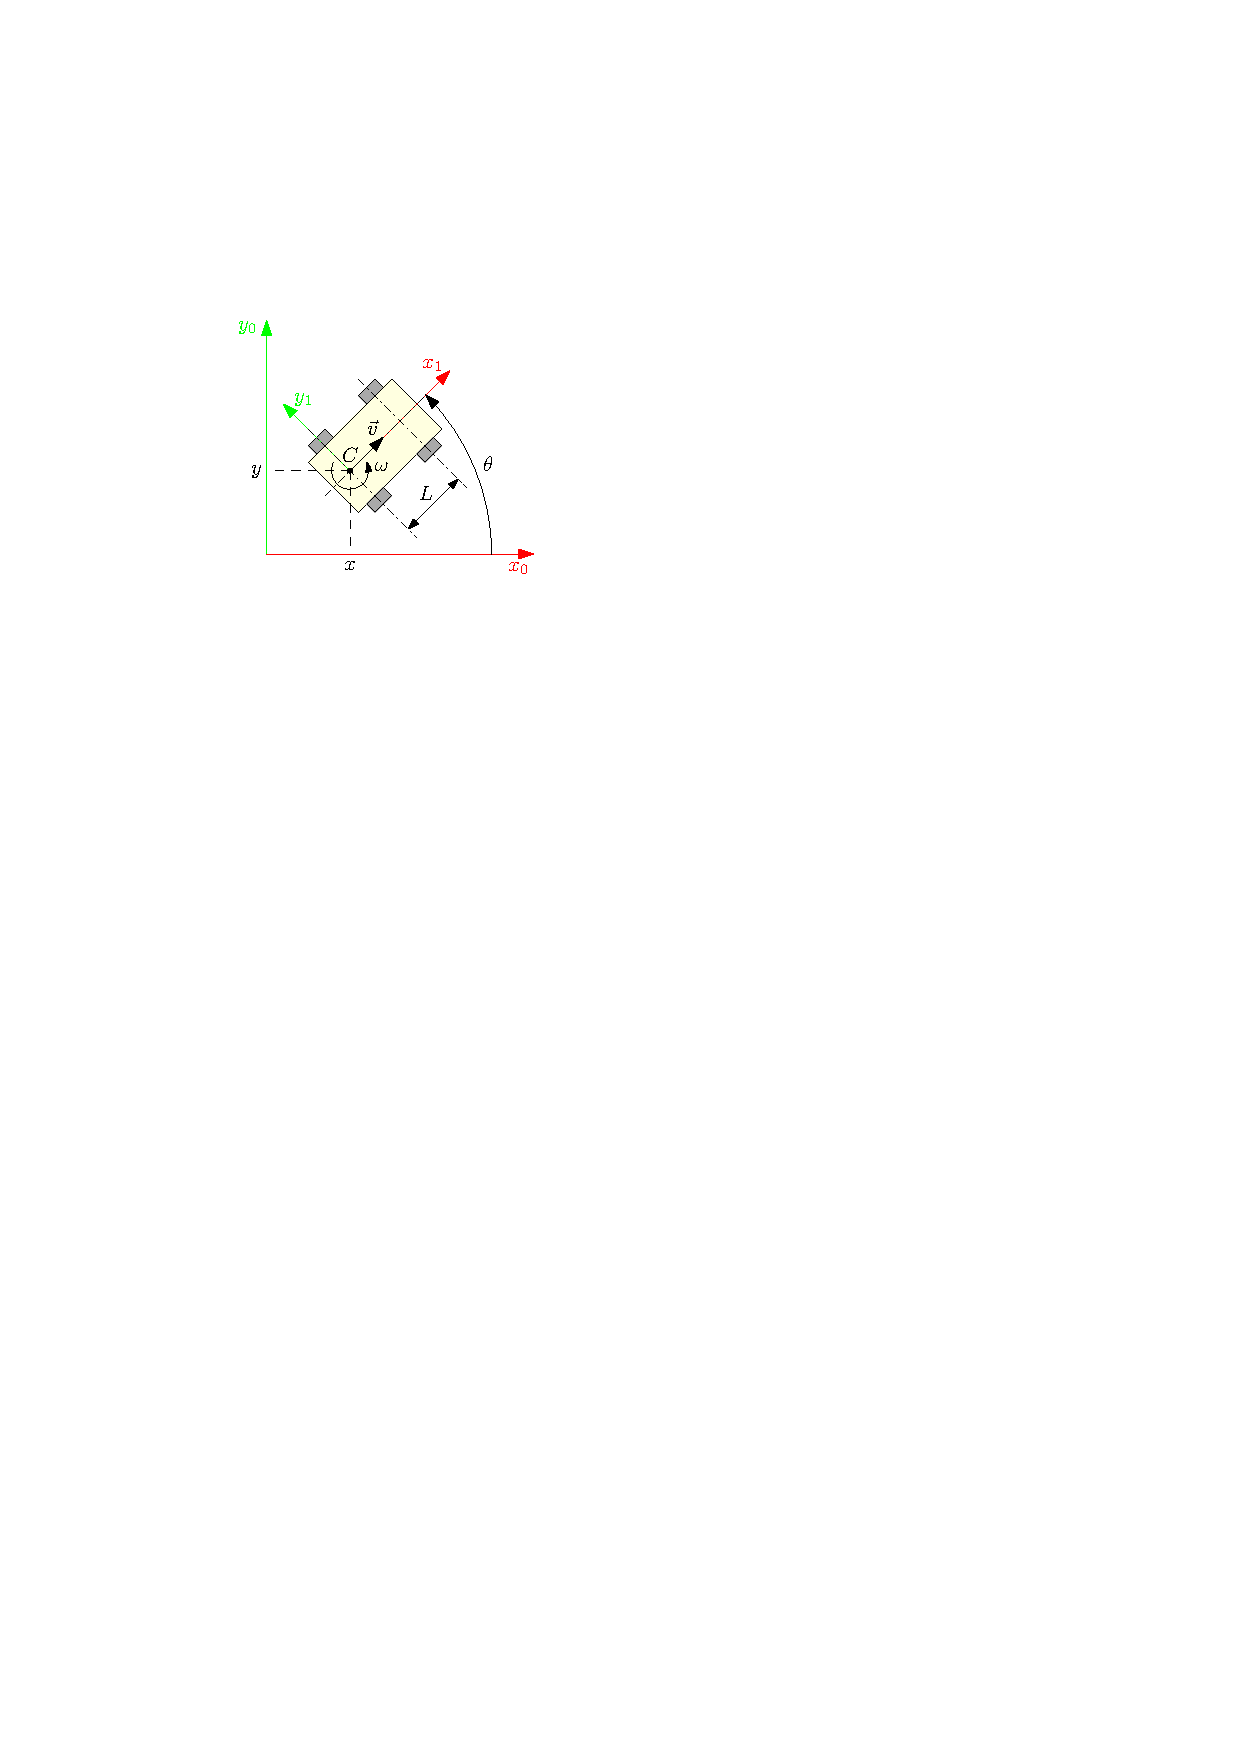
\includegraphics[width=0.5\textwidth]{kinematic_model_picture.pdf}
    \caption{Чертеж-пояснение к кинематической модели робота.}
    \label{img_kinematic_model_picture}
\end{figure}



\subsection{Локализация робота}
В~качестве угла~$\theta$ и угловой скорости~$\omega$ в работе использовались угол и угловая скорость, возвращаемые установленным на робота датчиком-гироскопом.
Координаты $x$ и $y$, в свою очередь, непосредственно не измерялись, а рассчитывались с использованием первых двух уравнений модели~\eqref{eq_robot_kinematic_model}.
При этом линейная скорость точки~$C$ с учетом третьего пункта перечня, представленного в разделе~\ref{part_robot_features}, определялась в соответствии со следующим выражением
\begin{equation}
    v = \underline{\omega} R,
\end{equation}
где $\underline{\omega}$~--- угловая скорость вращения вала тягового двигателя, $R$~--- радиус задних колес робота.

Состоятельность описанного принципа локализации робота была проверена с помощью сторонней системы технического зрения.
Подробности соответствующих экспериментов и полученные результаты доступны в Приложении~\ref{app_cv_system}.



\subsection{Структура системы управления}
Общая структура системы управления движением робота, позволяющая ему двигаться по желаемой траектории, показана на рисунке~\ref{img_control_system}.
Указанные на ней физические величины, ранее не упоминавшиеся в тексте данного отчета, значат следующее:
\begin{ESKDexplanation}
    \item $U_1$ ($U_2$)~--- напряжение, подаваемое на тяговый (рулевой) двигатель, выраженное в процентах от максимального напряжения (знак определяет направление вращения);
    \item $\bar\varphi$~--- угол поворота вала рулевого двигателя;
    \item $\bar{\varphi}_{min}$, $\bar{\varphi}_{max}$~--- его минимальное и максимальное значения ($\bar{\varphi}_{min} = -\bar{\varphi}_{max}$);
    \item $x_r$ и $y_r$~--- координаты, которые должен иметь робот в данный момент времени, чтобы следовать по желаемой траектории;
    \item $X_{des}$~--- желаемое значение величины~$X$.
\end{ESKDexplanation}

\vspace{0.5cm}

\begin{figure}[h]
    \centering
    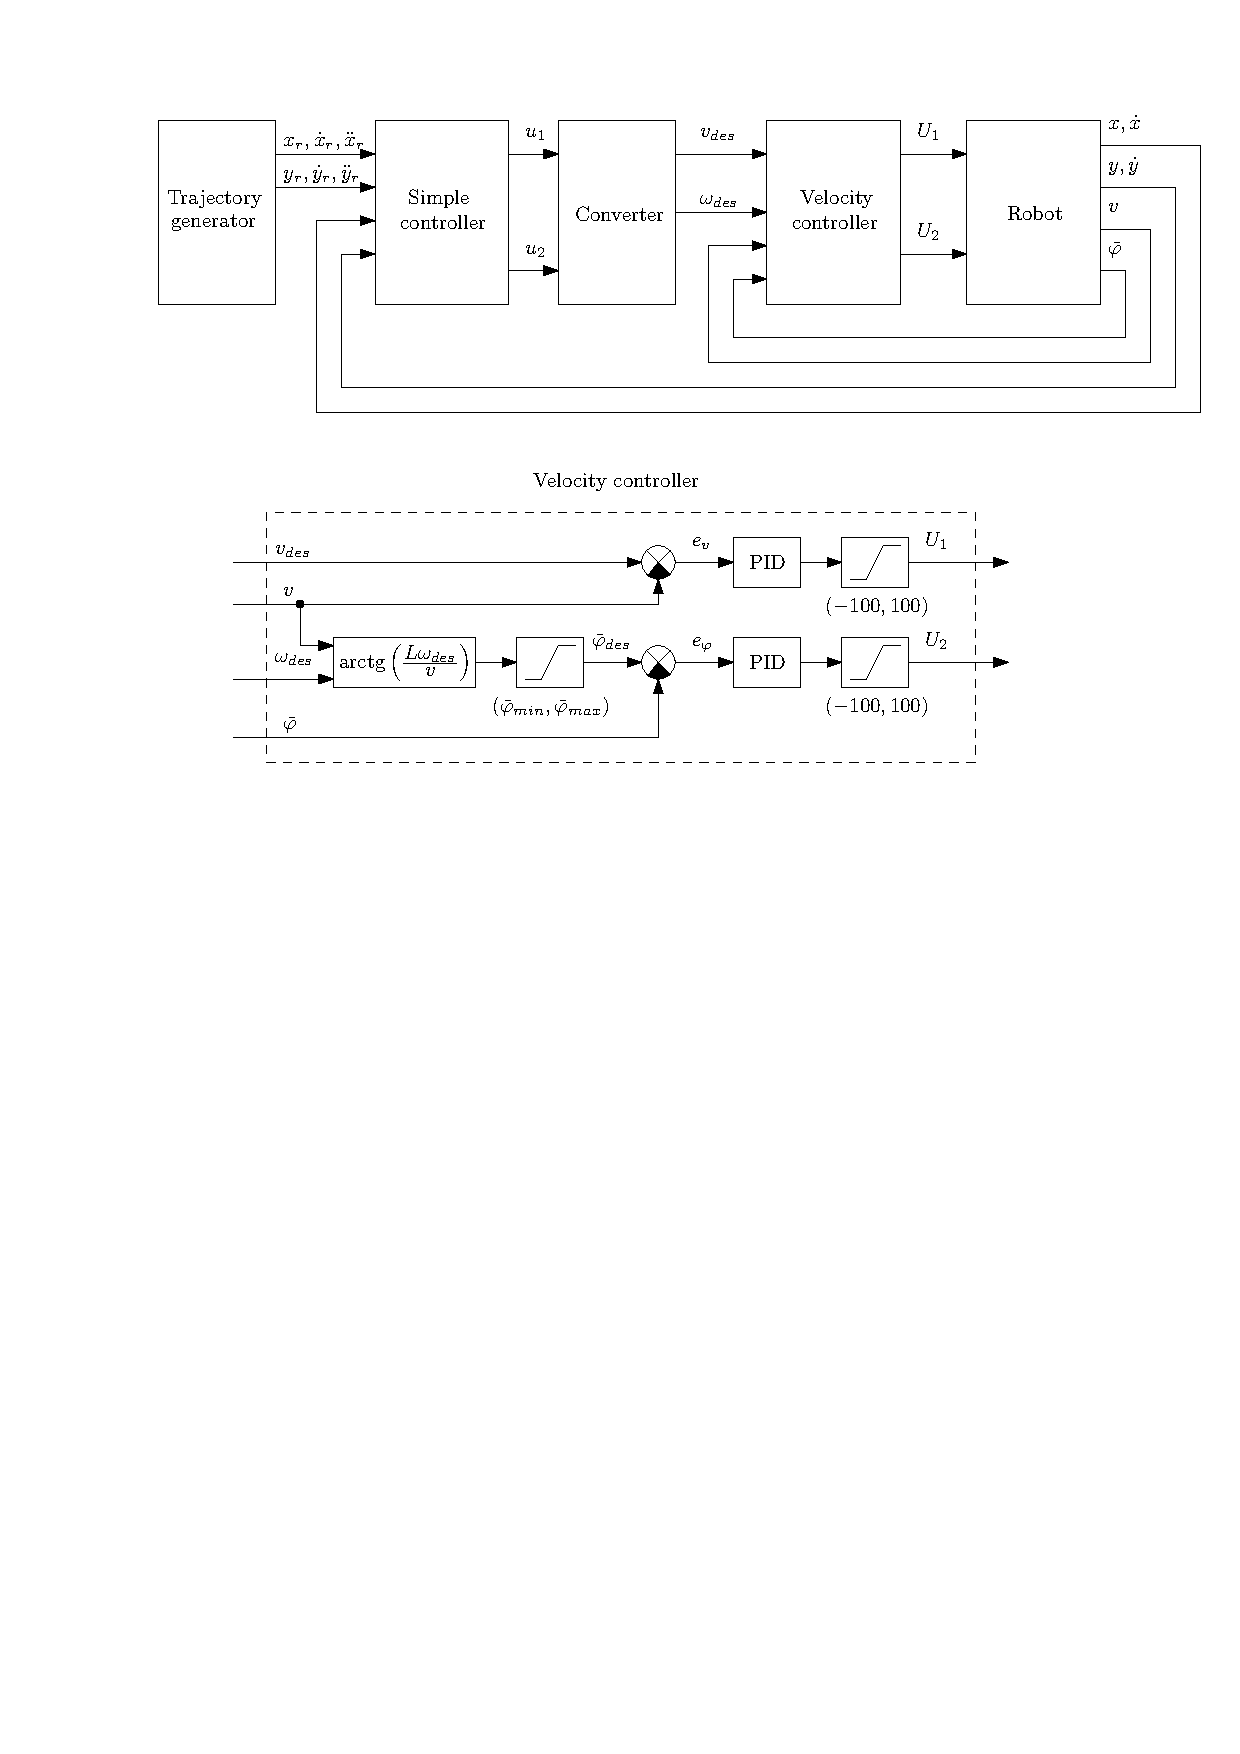
\includegraphics[width=\textwidth]{control_system.pdf}
    \vspace{0.0cm}
    \caption{Структура системы управления движением робота.}
    \label{img_control_system}
\end{figure}

Формирование желаемых значений для линейной и угловой скоростей робота блоком Converter, а также расчет <<предварительных>> управляющих воздействий в блоке Simple Controller производятся в соответствии со следующими выражениями~\cite{de_luca}:
\begin{equation}
    \left\{
    \begin{aligned}
        & \dot{\xi} = u_1 \cos \theta + u_2 \sin \theta, \\
        & v_{des} = \xi, \\
        & \omega_{des} = \frac{-u_1 \sin \theta + u_2 \cos \theta}{\xi},
    \end{aligned}
    \right.
\end{equation}
\begin{equation}
    \left\{
    \begin{aligned}
        & u_1 = \ddot{x}_r + k_{p1} (x_r - x) + k_{d1} (\dot{x}_r - \dot{x}), \\
        & u_2 = \ddot{y}_r + k_{p2} (y_r - y) + k_{d2} (\dot{y}_r - \dot{y})\ldotp
    \end{aligned}
    \right.
\end{equation}
